\section{\acl{LSTM}}
\textit{Daniel Andrés López, Frank Reichwein}

Eine weitere Art eine Klassifizierung vorzunehmen ist es ein neuronales Netz zu
verwenden. Dieser Ansatz ist durch die Biologie motiviert und lehnt sich an die
Arbeitsweise eines Gehirns an. Im Gehirn sind Neuronen über Synapsen iteinander
verbunden. Nervenbahnen aus dem gesamten Körper erreichen die Neuronen und
stimulieren sie in unterschiedlicher Intensität. Wird dabei ein Schwellwert
überschritten ist dieses Neuron aktiviert und sendet ebenfalls einen Impuls an
die mit ihm über die Synapsen verbundenen Neuronen. Dies geschieht fortlaufend.
Die Synapsen sind jedoch unterschiedlich stark ausgeprägt, um auch eine
unterschiedliche Stimulierungsintensität weiterzugeben. Dies kommt einer
Gewichtung der Neuronen gleich, da die Eingangssignale einen unterschiedlich
starken Einfluss auf das stimulierte Neuron haben. Die Synapsen sind jedoch
nicht fest und von vornerein vorgegeben. Sie werden kontinuerlich auf- und
abgebaut bzw. verändert. Diesen Vorgang wird im Allgemeinen Lernen bezeichnet.
Die erlebten Erfahrungen werden in dem Netz von Neuronen und Synapsen
verarbeitet und dadurch gespeichert. Erreichen das Gehirn nun neue
Sinneseindrücke werden die Neuronen erneut stimuliert und je nach Ergebnis
werden bestimmte Erinnerungen, Gefühle, Aktionen oder anderes erlebt und
ausgeführt. Jedoch sind sie nicht direkt an ein bestimmtes Ereignis geknüpft,
sondern wurden durch verschiedene Erfahrungen verallgemeinert, um so
verschiedenen Situationen gut verarbeiten zu können. 

\paragraph{Modelle von Neuronen und Synapsen}
Im Bereich des maschinellen Lernen wird versucht die Funktionsweise eines
Gehirns bzw. Netzes aus Neuronen und Synapsen nachzubilden. Dies wird durch
vereinfachte Modelle von Neuroen und Synapsen erreicht. Als Grundlage dient
dabei das Modell von McCulloch und Pitts von 1943 (vgl. \cite{Mcc43}). Es
modelliert ein Neuron mit $n$-vielen Eingabewerten ($x_1,\ldots,x_n$) und einem
Ausgabewert $y$. Die Eingabewerte entsprechen der Aktivierung eines
Vorgängerneurons und der Ausgabewert der Aktivierung des betrachteten Neurons.
\textbf{TODO Picture McCulloch and Pitts Neuron} Die \autoref{} zeigt den Aufbau
eines solchen Neurons. Die Eingaben weren dabei zuerst im \textit{Addierer}
summiert, eine Schwellwert (bzw. allgemeiner eine Aktivierungsfunktion) bestimmt
dann mit der Summe den Ausgabewert (die Aktivierung) des Neurons. De Weiteren
werden auch die Synapsen nachgebildet in dem jeder Eingabewert bei der
Summierung individuell gewichtet wird. Die Gewichte entsprechen den
unterschiedlich stark ausgeprägten Synapsen. Das klassische Modell erlaubt nur
binäre Ein- und Ausgaben, dies kann jedoch auf Reelle Zahlen erweitert werden,
um unterschiedlich starke Stimulierungen bzw. auch negative Werte (Hemmungen)
zuzulassen.

\paragraph{Neuronale Netzwerke}
Einzelne Neuronen können allerdings kein Gehrin nachbilden. Aus diesem Grund ist
di Kombination mehrerer Neuronen zu einem neuronalen Netz nötig. Im einfachsten
Fall entsteht dabei ein \textit{Perzeptron}. Es werden $n$-viele Neuronen
verwendet. Alle Eingaben werden von allen Neuronen verarbeitet und jedes Neuron
hat eine eigene Aktivierung. Die Gewichte (Synapsen) sind individuell für jedes
Neuron. Die Ausgaben ergeben den Ausgabevektor $\bf{y}$ des Netzwerkes. Um
komplexere Sachverhalte darstellen zu können ist es nötig Neuronen in
Abhängigkeit voneinander zu betrachten. Dies wird in \acp{MLP} vorgenommen.
Mehrere Perzeptrons werden hintereinandergeschaltet, sodass die Ausgabe des
einen Perzeptrons (ein Layer) die Eingabe des nächsten Perzeptrons ist.
Lediglich die Ausgabe des letzten Perzeptrons ist die Ausgabe des Netzwerks. 
Ein Netzwerk kann als gerichteter Graph dargestellt werden. Die Richtung
entspricht dem Datenfluss. Perzeptrons und \acp{MLP} sind azyklische Graphen,
d.h. die Verbindungen von Neuronen gehen nur in Vorwärtsrichtung und bilden
somit keinen Kreis. Daher werden diese Netzwerke \textit{Feedforward}-Netzwerke
genannt. Um besser die Funktionsweise von Gehirnen nachzubilden ist es
notwendig auch Verbidnungen von Neuronen auf sich selbst zuzulassen. Somit
entsteht ein zyklischer Graph und das Netzwerk wird zu einem Rekurrenten
Neuronalen Netz (\acsu{RNN}). 
\textbf{TODO Bilder von Neuronalen Netzen zur Verdeutlichung}

In den folgenden Kapiteln wird eine Sonderform von \acp{RNN} verwendet, ein
\ac{LSTM}. Dazu wird zuerst darauf eingegangen wie ein \ac{LSTM} im
Allgemeinen funktioniert und wie ein solches Netzwerk trainiert werden kann.
Darauf aufbauend wird das Verfahren auf das Projekt angepasst. Es werden die
Datenaufbereitung, die Anpassung des Klassifikators, die Implementierung in
Python, das Training und eine Evaluierung besprochen. 


 
\subsection{Funktionsweise des Klassifikators (Allgemein)}

 
\begin{figure}[htfp]
	\begin{center}
	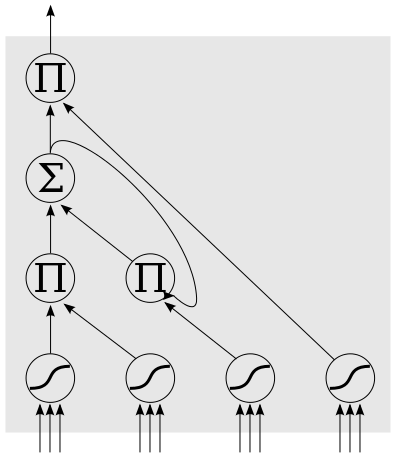
\includegraphics[width=0.3\textwidth]{lstm/lstm_block}
	\caption{Schema eines \acs{LSTM} Blocks}
	Quelle: \cite{WIKI2013}
	\label{fig:lstm_block}
	\end{center}
\end{figure}


\subsection{Anwednug auf Projekt}

\cite{schaul2010} 

\begin{lstlisting}[caption={Aufbau eines LSTM Netzes},label={lst:lstm_example}]{lst:lstm_example} 
net = buildNetwork(INPUTS, HIDDEN, OUTPUTS, hiddenclass=LSTMLayer,
outclass=SigmoidLayer, recurrent=True, bias=True) 
ds = DATASET 
trainer = BackpropTrainer(net, ds)
for _ in range(1000):
    trainer.train()
\end{lstlisting}



\subsubsection{Datenaufbereitung}
\label{sec:lstm_data}

\subsubsection{Anpassung des Klassifikators}
\subsubsection{Implementierung}

\subsubsection{Training}

\subsubsection{Evaluation}

\subsection{Fazit}


\nocite{GERS2001,WIKI2013,Schmidhuber2013,LSTM1,Nerbonne1}
